% ===================================================================== PARTE II
\chapter{Matemática mínima}
Este capítulo reúne las cinco herramientas que usa todo el proyecto. Si ya las
conoce, puede saltarlo.

\section{Vectores y matrices}
Un \term{vector} es una lista de números: $x = (x_1, x_2, \dots, x_N)$, uno por
entidad. Una \term{matriz} es una tabla: $W_{ij}$ es el número en la fila $i$ y la
columna $j$. Multiplicar una matriz por un vector, $(Wx)_i = \sum_j W_{ij}x_j$,
significa: para cada $i$, sumar lo que aporta cada $j$ ponderado por $W_{ij}$. En la
red de pagos, si $x_j$ es el déficit de $j$ y $W_{ij}$ lo que $j$ le paga a $i$, entonces
$(Wx)_i$ mide cuánto déficit le ``llega'' a $i$ desde quienes le pagan.

\section{Ecuaciones diferenciales}
Una \term{ecuación diferencial} dice cómo \emph{cambia} una cantidad. La más simple:
\[
\frac{dx}{dt} = -\alpha x \quad\Longrightarrow\quad x(t) = x(0)\,e^{-\alpha t}.
\]
Si hoy me falta $x(0)$, cada día corrijo una fracción $\alpha$ de lo que me falta y el
déficit decae exponencialmente. El tiempo típico de recuperación es $1/\alpha$.

\section{Integrar en el computador: Euler y RK4}
Casi nunca hay fórmula cerrada; se avanza en pasos pequeños $\Delta t$. El método de
\term{Euler} usa $x(t+\Delta t)\approx x(t) + \Delta t\, f(x(t))$. El proyecto usa
\term{Runge–Kutta de orden 4} (RK4): evalúa la pendiente cuatro veces dentro del paso
y las promedia; el error baja como $\Delta t^4$, así que con $\Delta t=0.01$ es
despreciable.

\begin{codigo}[label=src/finnet/integrate.py]
def rk4_step(dyn: Dynamics, x, theta, source, dt):
    k1x, k1t = dyn.rhs(x, theta, source)
    k2x, k2t = dyn.rhs(x + 0.5 * dt * k1x, theta + 0.5 * dt * k1t, source)
    k3x, k3t = dyn.rhs(x + 0.5 * dt * k2x, theta + 0.5 * dt * k2t, source)
    k4x, k4t = dyn.rhs(x + dt * k3x, theta + dt * k3t, source)
    x_new = x + (dt / 6.0) * (k1x + 2 * k2x + 2 * k3x + k4x)
    th_new = theta + (dt / 6.0) * (k1t + 2 * k2t + 2 * k3t + k4t)
    return x_new, th_new
\end{codigo}

\section{Valores propios}
Para un sistema lineal $\dot x = Mx$, la solución es una mezcla de ``modos''
$e^{\lambda t}v$, donde $Mv=\lambda v$: $\lambda$ es un \term{valor propio} y $v$ su
\term{vector propio}. Si todos los $\lambda$ tienen parte real negativa, todo decae
(estable); si alguno es positivo, algo crece sin control (inestable). Así, \emph{un
solo número}, el mayor valor propio, decide si la red amortigua o amplifica.

\section{Fases y números complejos}
Una fase $\theta$ es un ángulo: la posición de la aguja de un reloj. Se representa con
el número complejo $e^{i\theta}=\cos\theta + i\sin\theta$, un punto en el círculo
unitario. El promedio de muchos de esos puntos, $\frac1N\sum_j e^{i\theta_j}$, tiene
longitud $r\in[0,1]$: $r=1$ si todas las agujas apuntan igual (sincronía total),
$r\approx0$ si apuntan a cualquier lado.

% ---------------------------------------------------------------------------
\chapter{Tarea 1 · La red y el déficit}

\section{La matriz de pagos $W$}
Toda la información de la red está en la matriz $W$ de tamaño $N\times N$.
\begin{nota}[Convención única del proyecto]
$W_{ij}$ es el pago medio \textbf{de $j$ hacia $i$} por ciclo. Las filas suman lo que
recibe cada entidad, $k_i = \sum_j W_{ij}$ (su \emph{ingreso}); las columnas suman lo
que paga, $\mathrm{out}_j=\sum_i W_{ij}$. Los montos se normalizan para que el pago
medio sea 1: la unidad de dinero es ``un pago medio por ciclo''.
\end{nota}

\begin{figure}[h]
\centering
\begin{tikzpicture}[n/.style={circle,draw=azul,fill=azul!10,minimum size=8mm,font=\sffamily},
  e/.style={-{Stealth[length=2.5mm]},thick}]
\node[n] (1) at (0,0) {1};
\node[n] (2) at (2.4,0.9) {2};
\node[n] (3) at (2.4,-0.9) {3};
\draw[e] (1) -- node[above,font=\small]{3} (2);
\draw[e] (2) -- node[right,font=\small]{1} (3);
\draw[e] (3) -- node[below,font=\small]{2} (1);
\node at (7,0) {$W=\begin{pmatrix}0&0&2\\3&0&0\\0&1&0\end{pmatrix}
\quad\begin{array}{l}\text{fila } i\text{: lo que recibe } i\\
\text{columna } j\text{: lo que paga } j\end{array}$};
\end{tikzpicture}
\caption{Una red de tres entidades. La entidad 1 le paga 3 a la 2, así que $W_{21}=3$.}
\end{figure}

\section{Formas de red}
\archivo{src/finnet/networks.py} genera tres familias clásicas:
\begin{itemize}
\item \term{Erdős–Rényi}: cada par se conecta al azar con la misma probabilidad. Es la
referencia ``sin estructura''.
\item \term{Barabási–Albert}: los nodos nuevos prefieren conectarse con los que ya
tienen muchas conexiones; aparecen ``hubs'' (como los grandes bancos).
\item \term{Núcleo-periferia}: un núcleo pequeño y denso (bancos grandes) y una
periferia que se conecta sobre todo con el núcleo. Es la forma observada en sistemas
de pagos reales.
\end{itemize}
Los montos son $W_{ij}=\sqrt{s_is_j}\,\varepsilon_{ij}$, con tamaños $s$ y ruido
$\varepsilon$ lognormales (pocos montos muy grandes, muchos pequeños):
\begin{codigo}[label=src/finnet/networks.py · generate]
sizes = rng.lognormal(0.0, cfg.amount_sigma, cfg.n)
noise = rng.lognormal(0.0, cfg.amount_sigma, (cfg.n, cfg.n))
W = np.where(A, np.sqrt(np.outer(sizes, sizes)) * noise, 0.0)
return normalize_weights(W)
\end{codigo}

\section{La ecuación del déficit}
La primera versión del modelo es lineal:
\[
\boxed{\;\frac{dx_i}{dt} = -\alpha\,x_i + \beta\sum_j W_{ij}\,x_j\;}
\]
\begin{itemize}
\item $-\alpha x_i$: \textbf{autocorrección}. Cada entidad corrige una fracción
$\alpha$ de su déficit por ciclo.
\item $\beta\sum_j W_{ij}x_j$: \textbf{contagio}. Si quien me paga está en déficit, me
paga menos o más tarde, y eso me crea déficit, en proporción a cuánto me paga
($W_{ij}$).
\end{itemize}

\section{El índice de amplificación $R$}
En forma matricial, $\dot x = (-\alpha I + \beta W)x$. Como $W$ no tiene números
negativos, el teorema de \term{Perron–Frobenius} garantiza que su valor propio más
grande es real y positivo: el \term{radio espectral} $\rho(W)$. El sistema es estable
si y solo si $-\alpha + \beta\rho(W) < 0$, es decir
\[
\boxed{\;R = \frac{\beta\,\rho(W)}{\alpha} < 1.\;}
\]
\begin{idea}
$R$ compara dos fuerzas: cuánto se contagia el déficit por la red ($\beta\rho$) contra
cuánto se corrige solo ($\alpha$). Es el análogo del ``número de reproducción'' de una
epidemia: con $R<1$ cada problema genera menos de un problema nuevo y se apaga.
\end{idea}

\begin{codigo}[label=src/finnet/spectral.py]
def perron_root(W: np.ndarray) -> float:
    """Valor propio dominante ρ(W) (real y no negativo para W >= 0)."""
    ev = np.linalg.eigvals(np.asarray(W, dtype=float))
    return float(np.max(ev.real)) if ev.size else 0.0

def amplification_index(W: np.ndarray, params: Params) -> float:
    """Índice de amplificación ``R = β ρ(W) / α``."""
    num = params.beta * perron_root(W)
    ...
    return num / params.alpha
\end{codigo}

Además, los vectores propios dominantes ordenan a las entidades: el vector
\emph{izquierdo} mide cuánto déficit \emph{propaga} cada una (importancia) y el
\emph{derecho} cuánto \emph{acumula} (vulnerabilidad).

\section{Parámetros y el modelo como objeto}
\archivo{src/finnet/model.py} define \texttt{Params}, un contenedor inmutable de los
parámetros: $\alpha,\beta$ (tarea 1), $D_0$ (tarea 2), $K,\gamma,\omega$ (tarea 3),
umbrales y pérdida $\lambda$ (tarea 4). Todos los términos nuevos valen cero por
defecto: \textbf{con los términos apagados, el modelo vuelve exactamente al de la
tarea anterior}. Esta regla de diseño es la que permite construir en capas y probar
cada capa por separado.

% ---------------------------------------------------------------------------
\chapter{Tarea 2 · Difusión y estabilidad}

\section{El Laplaciano: mover sin crear ni destruir}
La tarea 2 agrega la \term{redistribución}: la presión de liquidez se traslada por la
red (por ejemplo, alguien presta a quien le falta), pero el total no cambia. Eso lo
hace el \term{Laplaciano de flujo}
\[
L = D_\text{out} - W,\qquad \frac{dx}{dt} = -D_0\,L\,x,
\]
con $D_\text{out}$ la matriz diagonal de pagos salientes. Las columnas de $L$ suman
cero, por eso $\sum_i x_i$ se conserva: la difusión mueve déficit, no lo crea.

\section{El modelo con las dos piezas}
\[
\dot x = M x,\qquad M = -\alpha I - D_0 L + \beta W.
\]
\begin{itemize}
\item \term{Estabilidad} $\sigma = \max\mathrm{Re}\,\lambda(M)$: si $\sigma<0$ la red
se recupera de cualquier choque.
\item \term{Tiempo de recuperación} $\tau_\text{rec} = -1/\sigma$ (en ciclos).
\item \term{Conectividad algebraica} $\lambda_2$: el segundo valor propio del
Laplaciano simétrico. Mide qué tan bien conectada está la red; en redes simétricas
la tasa de recuperación es exactamente $\alpha + D_0\lambda_2$.
\end{itemize}

\section{Comunidades}
El vector propio asociado a $\lambda_2$ (vector de \term{Fiedler}) parte la red en dos
grupos poco conectados entre sí; repitiendo la partición se obtienen
\term{comunidades}. Se usa la versión \emph{normalizada} del Laplaciano (corte
normalizado de Shi y Malik, 2000), que da grupos balanceados en lugar de separar
unos pocos nodos periféricos.

\begin{codigo}[label=src/finnet/spectral.py]
def stability(W: np.ndarray, params: Params) -> float:
    """``σ = max Re λ(M)``; el sistema lineal es estable si σ < 0."""
    return float(spectrum(linear_operator(W, params))[0].real)

def recovery_time(W: np.ndarray, params: Params) -> float:
    """``τ_rec = -1/σ`` en ciclos; ``inf`` si σ >= 0 (no se recupera)."""
    sigma = stability(W, params)
    return -1.0 / sigma if sigma < 0 else float("inf")
\end{codigo}

% ---------------------------------------------------------------------------
\chapter{Tarea 3 · Sincronización: el modelo de Kuramoto}

\section{Osciladores}
Cada entidad tiene un ciclo de pagos, representado por una fase $\theta_i(t)$ que
avanza a su ritmo natural $\omega_i$ (una vuelta completa, $2\pi$, por ciclo). Si
dependo de los fondos de otros, ajusto mi ritmo al de ellos:
\[
\boxed{\;\frac{d\theta_i}{dt} = \omega_i + \frac{K}{\langle k\rangle}\sum_j W_{ij}\,
\sin(\theta_j-\theta_i)\;}
\]
El término $\sin(\theta_j-\theta_i)$ acelera a $i$ si $j$ va adelante y lo frena si va
atrás. $K$ es la fuerza del acople.

\section{Parámetro de orden y coherencia local}
\[
r = \Big|\frac1N\sum_j e^{i\theta_j}\Big|,\qquad
r_i = \frac{1}{k_i}\sum_j W_{ij}\cos(\theta_j-\theta_i).
\]
$r$ mide la sincronía global; $r_i$ mide si a la entidad $i$ el dinero le llega
\emph{en fase} ($r_i\approx1$) o desfasado ($r_i\le0$) respecto a su propio ciclo.

El resultado clásico de Kuramoto: con frecuencias repartidas según una distribución
de Lorentz de ancho $\Delta$, en la red completa hay sincronía parcial a partir de
$K_c=2\Delta$, con $r=\sqrt{1-2\Delta/K}$. El proyecto lo reproduce numéricamente (ver
capítulo de validación).

\section{La desincronización cuesta}
El puente entre el ritmo y el déficit es un término nuevo en la ecuación de $x$:
\[
\gamma\,k_i\,(1-r_i) = \gamma\sum_j W_{ij}\big(1-\cos(\theta_j-\theta_i)\big).
\]
Es el ingreso que llega desfasado, multiplicado por $\gamma$. Si todo llega en fase,
el término es cero; si llega en contrafase, cuesta $2\gamma k_i$.

\begin{nota}[Dos diferencias deliberadas con la propuesta]
(1) El acople se divide por el ingreso medio $\langle k\rangle$ y no por $N$: en redes
dispersas, $K/N$ hace desaparecer el acople cuando $N$ crece (forma de Rodrigues et
al., 2016). En la red completa ambas coinciden. (2) El término de desincronización es
proporcional al ingreso desfasado, no un número fijo: así es dimensionalmente
consistente (dinero por ciclo).
\end{nota}

\section{El modelo completo}
\[
\frac{dx_i}{dt} = -\alpha x_i + \beta\sum_j W_{ij}x_j - D_0(Lx)_i + \gamma k_i(1-r_i)
+ \eta_i(t),
\]
\[
\frac{d\theta_i}{dt} = \omega_i + \frac{K}{\langle k\rangle}\sum_j W_{ij}
\sin(\theta_j-\theta_i).
\]
En el código, todo el lado derecho se evalúa con \emph{un solo} producto de matrices
$W\,[x,\cos\theta,\sin\theta]$, lo que lo hace rápido:
\begin{codigo}[label=src/finnet/model.py · Dynamics.rhs]
c, s = np.cos(theta), np.sin(theta)
prod = self.W @ np.column_stack((x, c, s))
Wx, zr, zi = prod[:, 0], prod[:, 1], prod[:, 2]
dx = -self.diag * x + self.offdiag * Wx + source
if self.p.gamma > 0:
    # k_i (1 - r_i) = k_i - Σ_j W_ij cos(θ_j - θ_i)
    dx = dx + self.p.gamma * (self.k - (c * zr + s * zi))
# Im(e^{-iθ} z) = cos θ · Im z - sin θ · Re z
dth = self.omega + self.kur * (c * zi - s * zr)
\end{codigo}

% ---------------------------------------------------------------------------
\chapter{Tarea 4 · Impagos y cascadas}

\section{El umbral}
Cada entidad tiene un \term{colchón} $x_i^{(c)}$: un múltiplo de sus pagos salientes,
con algo de dispersión aleatoria. Si $x_i > x_i^{(c)}$, la entidad cae en impago:
\begin{enumerate}
\item deja de pagar: su columna en $W$ se anula;
\item quienes recibían de ella pierden ese ingreso, lo que les suma déficit
(parámetro $\lambda$, la pérdida);
\item esos saltos pueden hacer caer a otros \emph{en el mismo instante}, así que se
repite hasta que no aparece ningún impago nuevo (cascada instantánea).
\end{enumerate}

\begin{codigo}[label=src/finnet/integrate.py · simulate (detección de impagos)]
def detect_defaults(t: float) -> bool:
    """Aplica impagos (y sus saltos) hasta agotar la cascada instantánea."""
    if thresholds is None:
        return False
    changed = False
    while True:
        new = ~defaulted & (x > thresholds)
        if not new.any():
            return changed
        apply_defaults(np.flatnonzero(new), t, None)
        changed = True
\end{codigo}

\section{Choques}
\begin{itemize}
\item \term{Retiro de liquidez}: un salto en el déficit de la entidad chocada.
\item \term{Caída operativa}: la entidad recibe pero no paga durante $T$ ciclos (una
falla tecnológica); si no cruza su umbral, se recupera.
\item \term{Quiebra} (agregado en la tarea 6): la entidad cae en impago en $t_0$.
\end{itemize}

\section{Modelos clásicos de comparación}
\archivo{src/finnet/cascades.py} implementa tres modelos de la literatura para
contrastar con la dinámica:
\begin{itemize}
\item \term{Eisenberg y Noe (2001)}: qué fracción de sus deudas puede pagar cada
entidad cuando todas pagan lo máximo posible a la vez (vector de liquidación).
\item \term{DebtRank} (Battiston et al., 2012): cuánto estrés propaga una entidad, sin
contar dos veces el mismo camino.
\item \term{Watts (2002)}: una entidad cae si cae una fracción suficiente de sus
pagadores.
\end{itemize}

\section{Indicadores de riesgo}
\archivo{src/finnet/metrics.py} resume cada corrida: fracción de entidades en impago,
liquidez no pagada acumulada, tiempo hasta el primer contagio, colapso global (cae al
menos el 30~\%) e \term{importancia sistémica} de cada entidad (fracción media de
\emph{otras} que caen cuando se la choca).

% ---------------------------------------------------------------------------
\chapter{Tarea 5 · Experimentos y aprendizaje automático}

\section{Por qué aprender}
Simular un escenario tarda del orden de 0.1~s. Responder ``¿qué tan riesgosa es cada
entidad?'' exige simular un choque a cada una. Un modelo de aprendizaje automático
entrenado con miles de simulaciones responde en milisegundos.

\section{El dataset}
\archivo{src/finnet/experiments.py} corre la dinámica completa a partir de
\archivo{configs/sweep.yaml}:
\begin{itemize}
\item 300 redes (de 30 a 150 entidades, las tres topologías);
\item 20\,000 escenarios muestreados con un \term{hipercubo latino} (cubre el espacio
de 13 parámetros de forma pareja) y con más densidad cerca de $R=1$, donde ocurre la
transición;
\item una tabla por entidad con su tamaño de cascada cuando el choque empieza en ella.
\end{itemize}
Cada fila tiene su propia semilla: el dataset es \textbf{reproducible bit a bit}, sin
importar en qué orden ni con cuántos procesos se genere. Se guarda en formato
\term{Parquet} con un esquema validado (columnas, tipos y rangos).

\section{Los modelos}
\begin{itemize}
\item \term{Regresión logística}: el modelo más simple de probabilidad; una suma
ponderada de variables pasada por una curva en forma de S.
\item \term{XGBoost}: muchos árboles de decisión pequeños que se corrigen unos a otros
(\emph{gradient boosting}). Suele ser el mejor en datos tabulares.
\item \term{GCN} (Kipf y Welling, 2017): una red neuronal que trabaja directamente
sobre el grafo; cada nodo combina su información con la de sus vecinos.
\item \term{PINN} (Raissi et al., 2019): una red neuronal ``informada por la física''
que recupera los parámetros $\alpha,\beta,\gamma,K$ a partir de trayectorias, obligando
a que respete las ecuaciones del modelo.
\end{itemize}

\section{Evaluar sin hacer trampa}
\begin{itemize}
\item \term{GroupKFold por red}: se divide en 5 partes de modo que una misma red
nunca esté a la vez en entrenamiento y en prueba. Si no, el modelo ``memoriza'' la red.
\item \term{ROC-AUC}: probabilidad de que el modelo ponga a un caso positivo
por encima de uno negativo (0.5 = azar, 1 = perfecto).
\item \term{PR-AUC}: útil cuando los positivos son pocos.
\item \term{Brier} y \term{calibración}: si el modelo dice ``30~\%'', ¿ocurre el 30~\%
de las veces?
\item \term{SHAP}: cuánto aporta cada variable a cada predicción.
\end{itemize}

% ---------------------------------------------------------------------------
\chapter{Tarea 6 · Riesgo crediticio en una red multicapa}

\section{De entidades a clientes}
Las tareas 1–5 estudian una red de entidades abstractas. La tarea 6 baja al nivel de
los \textbf{clientes de un banco}. Hay dos tipos de nodo y tres capas de relaciones:

\begin{center}
\begin{tabular}{llll}
\toprule
Capa & Dirección & Ciclo & Contagio \\
\midrule
N · nómina & firma $\to$ persona & quincenal o mensual & la firma cae, cae el sueldo \\
S · proveedores & firma $\to$ firma & facturas & el cliente no paga al proveedor \\
T · transferencias & persona $\to$ persona & irregular & débil y difuso \\
\bottomrule
\end{tabular}
\end{center}

\begin{figure}[h]
\centering
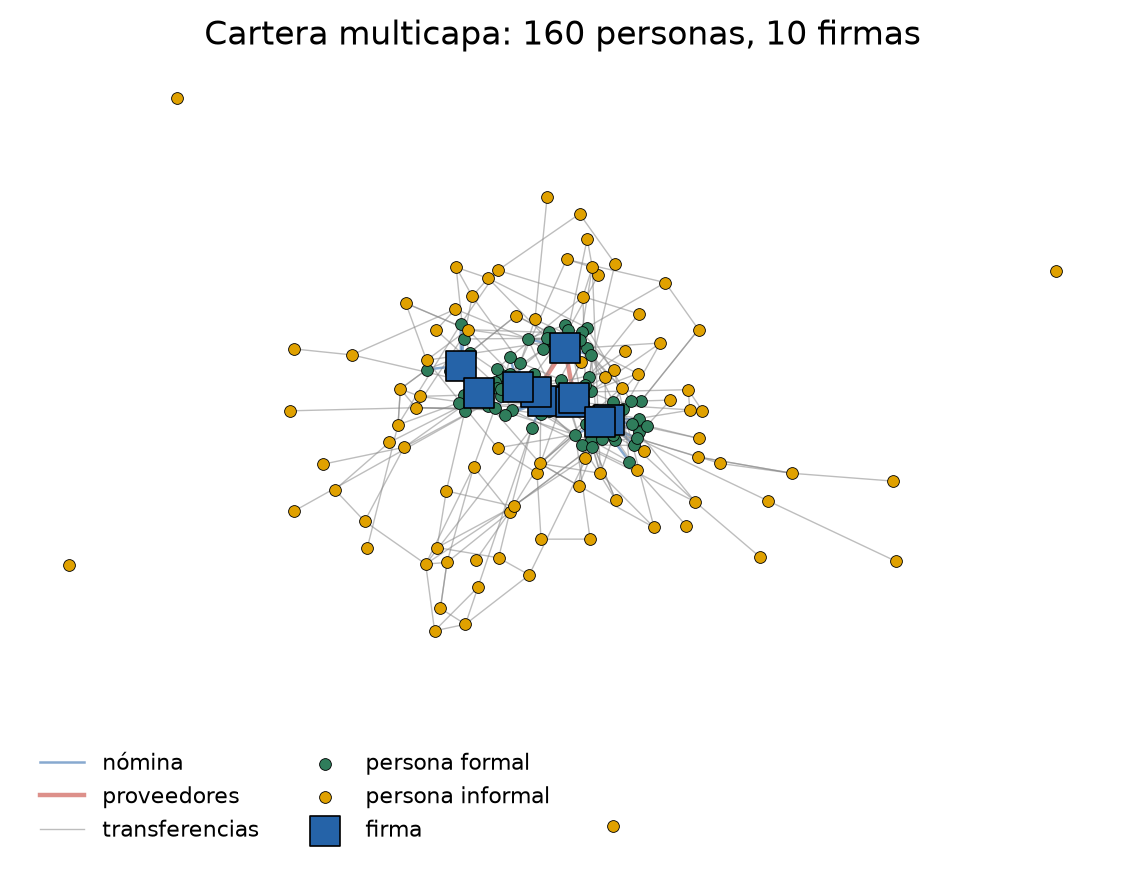
\includegraphics[width=0.85\textwidth]{tarea6_red_multicapa.png}
\caption{Una cartera pequeña. Cuadrados: firmas; círculos verdes: personas con
empleo formal; ámbar: informales. Azul: nómina; rojo: proveedores; gris:
transferencias.}
\end{figure}

\section{El mundo sintético: \texttt{finnet.world}}
No hay datos públicos con la red de pagos de los clientes de un banco, así que se
\emph{genera} una cartera realista con un mecanismo conocido. Eso permite comprobar
que el método recupera lo que debe.

\begin{itemize}
\item \archivo{world/entities.py}: 2000 personas y 100 firmas.
  \begin{itemize}
  \item 55~\% de las personas son informales (sin empleador en la red), del orden de
  la informalidad en Colombia según el DANE.
  \item El tamaño de las firmas sigue una ley de Pareto: pocas firmas grandes emplean
  a mucha gente.
  \item Variables clásicas: ingreso (en salarios mínimos por mes), endeudamiento,
  edad, antigüedad en el banco, número de productos, moras en 12 meses, empleo formal.
  \item Ritmos: las firmas pagan nómina mensual o quincenal; los formales heredan el
  ritmo de su empleador con poca dispersión; los informales tienen ritmos dispersos.
  \end{itemize}
\item \archivo{world/layers.py}: construye las tres capas. La nómina conecta a cada
formal con su único empleador; los proveedores siguen una matriz insumo-producto
entre sectores; las transferencias prefieren compañeros de trabajo y personas de la
misma comunidad.
\item \archivo{world/transactions.py}: el registro de pagos (más abajo).
\end{itemize}

\subsection{La verdad del terreno}
Cada cliente tiene una PD anual verdadera:
\[
\mathrm{logit}(\mathrm{PD}_i) = b + \sum_k c_k\,z_k(i) + \sigma_u\,u_i,
\]
donde $z_k$ son las variables clásicas estandarizadas y $u_i$ un componente
\emph{latente} que ningún dato muestra del todo (la mora observada lo revela solo en
parte, como el historial real). $b$ se ajusta para que la PD media sea 5~\% en personas
y 3~\% en firmas. Estas columnas se llaman \texttt{truth\_*} y una regla del código
impide que lleguen a un modelo:

\begin{codigo}[label=src/finnet/schema.py]
def assert_no_truth(columns) -> None:
    """Falla si alguna columna es verdad del terreno (fuga de información)."""
    leaked = [c for c in columns if str(c).startswith(TRUTH_PREFIX)]
    if leaked:
        raise ValueError(
            f"Columnas de verdad del terreno no pueden entrar a un modelo: {leaked}"
        )
\end{codigo}

\section{El motor multicapa}
El motor de las tareas 1–4 se generaliza sin romperlo. Con varias capas $\ell$ y el
tiempo medido en \textbf{meses}:
\[
\dot x_i = -\alpha x_i + \sum_\ell \beta_\ell\sum_j\frac{W^\ell_{ij}}{s_i}x_j
+ \gamma\,\frac{k_i}{s_i}(1-r_i) + \sigma\,\xi_i(t),
\]
\[
\dot\theta_i = \omega_i + \sum_\ell K_\ell \sum_j \frac{W^\ell_{ij}}{k_i}\sin(\theta_j-\theta_i).
\]
\begin{itemize}
\item $x_i$ ahora es \textbf{adimensional}: el déficit como fracción del ingreso total
$s_i$ (que incluye lo que llega de fuera de la red). Así una persona y una empresa son
comparables.
\item Cada capa tiene su propio contagio $\beta_\ell$ y su propio acople $K_\ell$.
\item El acople de fase se normaliza por fila: cada cliente ajusta su ritmo según la
participación de cada pagador en su ingreso.
\item $\sigma\xi_i(t)$ es ruido: pequeños choques de liquidez aleatorios (integrado con
el esquema de Euler–Maruyama).
\item El colchón depende de la PD verdadera,
$x_i^{(c)} = c\,(\mathrm{PD}_\text{ref}/\mathrm{PD}_i)^{\kappa}\,\varepsilon_i$: quien
es más riesgoso tiene menos margen.
\item Impagos \textbf{idiosincráticos}: cada cliente cae por sus propias razones en un
instante aleatorio con tasa $-\ln(1-\mathrm{PD}_i)/12$ por mes.
\end{itemize}

En el código, estas matrices se empaquetan en un objeto \texttt{Coupling}. Si no se
pasa, el motor es \emph{bit a bit} el de la versión 1 (lo verifica una prueba):
\begin{codigo}[label=src/finnet/model.py · Dynamics.\_rhs\_coupled]
cpl = self.coupling
dx = -self.p.alpha * x + cpl.stress @ x + source
if not self.need_phases:
    return dx, self.omega
c, s = np.cos(theta), np.sin(theta)
cs = np.column_stack((c, s))
if self.p.gamma > 0:
    zw = self.W @ cs
    # (k_i / s_i)(1 - r_i) = (k_i - Σ_j W_ij cos(θ_j - θ_i)) / s_i
    dx = dx + self.gamma_scale * (self.k - (c * zw[:, 0] + s * zw[:, 1]))
zc = cpl.phase @ cs
dth = self.omega + (c * zc[:, 1] - s * zc[:, 0])
\end{codigo}
Las matrices son \term{dispersas} (\texttt{scipy.sparse}): con 2100 clientes hay unas
5\,000 relaciones y no 4.4 millones de casillas, y una cartera completa se simula en
menos de un segundo.

\section{Lo que ve el banco: el registro de transacciones}
El banco no ve fases ni ritmos naturales. Ve \emph{pagos con fecha}. El simulador los
produce así: cada vez que la fase de un pagador cruza un múltiplo de $2\pi$, ejecuta
su ciclo de pagos y paga a cada receptor (más un pequeño ruido en el día y el monto) y
paga su cuota al banco. Quien cae en impago deja de pagar.

\section{Estimar desde las transacciones}
\archivo{src/finnet/credit/estimate.py} hace lo que haría un analista con los datos
reales:
\begin{enumerate}
\item $\hat W$: cuánto le paga cada pagador a cada receptor por mes (mientras pagó).
\item \textbf{Fase por eventos} (Pikovsky, Rosenblum y Kurths, 2001): si $t_k$ son los
instantes de los ciclos de pago de un cliente,
\[
\hat\theta(t) = 2\pi\Big(k + \frac{t-t_k}{t_{k+1}-t_k}\Big),\qquad t_k\le t<t_{k+1}.
\]
\item $\hat r_i(t)$: la coherencia local con las fases estimadas de sus pagadores.
\end{enumerate}
\begin{codigo}[label=src/finnet/credit/estimate.py · event\_phase]
k = np.searchsorted(times, grid, side="right") - 1
inside = (k >= 0) & (k < times.size - 1)
ki = k[inside]
theta[inside] = TWO_PI * (
    ki + (grid[inside] - times[ki]) / (times[ki + 1] - times[ki])
)
\end{codigo}

\begin{figure}[h]
\centering
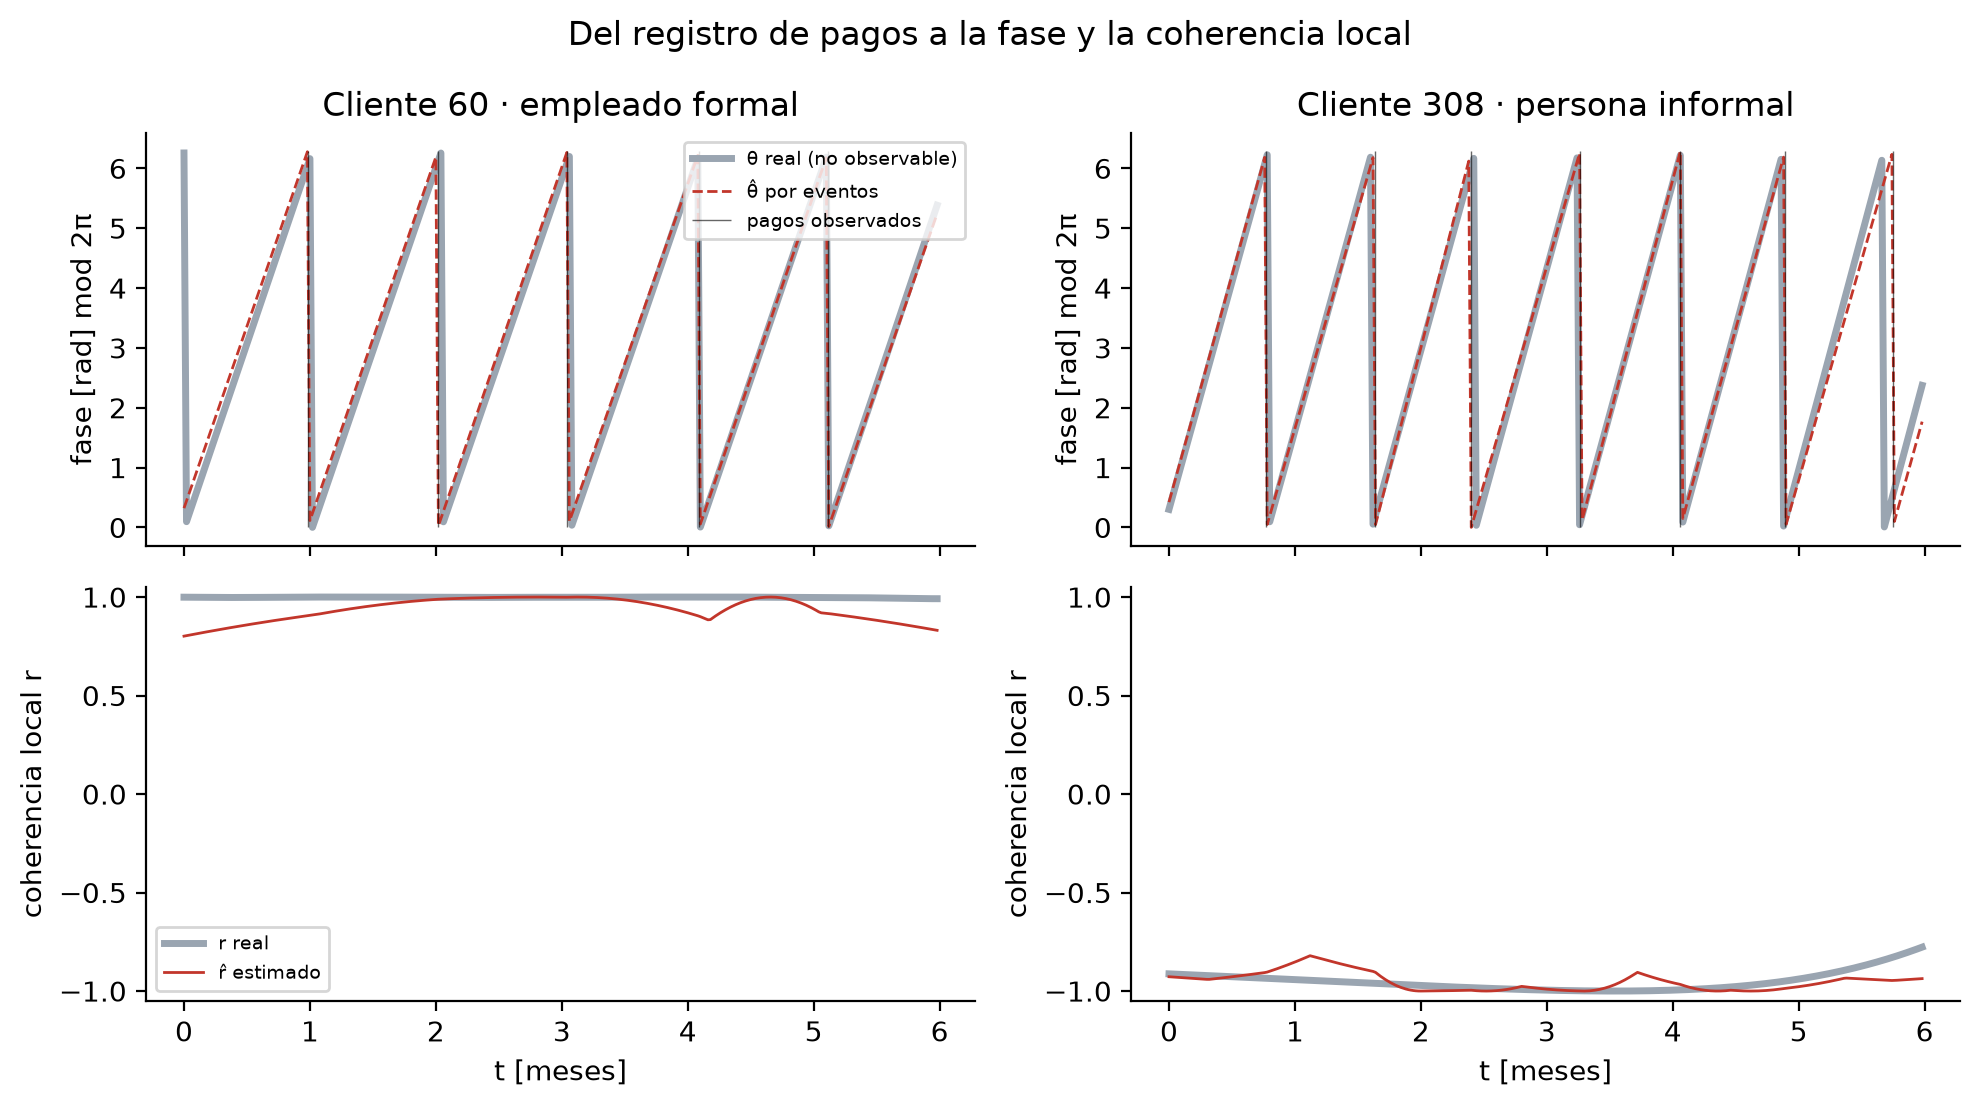
\includegraphics[width=\textwidth]{tarea6_fase_eventos.png}
\caption{Arriba: la fase real (gris, no observable) y la estimada solo con los pagos
(rojo), para un empleado formal y una persona informal. Abajo: su coherencia local
real y estimada. El formal está en fase con su empleador ($r\approx1$); la informal
recibe en contrafase ($r\approx-1$): el dinero le llega justo cuando no le sirve.}
\end{figure}

\section{Tres niveles de variables}
\archivo{src/finnet/credit/features.py} construye, para cada cliente y solo con los
primeros 6 meses de datos:
\begin{description}
\item[1 · Clásico.] Ingreso, endeudamiento, edad, antigüedad, productos, moras, empleo
formal, tamaño (firmas). Lo que usa cualquier score.
\item[2 · + Red estática.] Qué parte del ingreso llega por nómina, proveedores o
transferencias; número de pagadores; concentración del ingreso; PageRank; tamaño,
endeudamiento y moras del empleador; riesgo medio de los pagadores. Es lo que ya
explora la literatura.
\item[3 · + Red dinámica.] Coherencia local media $\hat r$, su variabilidad, tiempo
desincronizado ($\hat r<0.5$), desfase con los pagadores, desajuste de ritmo,
irregularidad de los ciclos propios y de los pagadores, e ingreso de pagadores que
dejaron de pagar. \textbf{Este es el aporte.}
\end{description}
La etiqueta es: ¿el cliente cae en impago en los 12 meses siguientes? Quien ya cayó
durante la observación se excluye.

\section{Evaluar con un control}
\archivo{src/finnet/credit/evaluate.py} y \archivo{experiment.py}:
\begin{itemize}
\item \textbf{Dos mundos}. En el mundo \emph{con red} los acoples están encendidos. En
el mundo \emph{nulo} ($\beta_\ell=\gamma=\lambda=0$) la red no crea déficit, pero los
clientes, las redes y \emph{todos los sorteos aleatorios} son idénticos (cuatro flujos
aleatorios independientes derivados de la misma semilla). Si en el mundo nulo las
variables de red ``mejoraran'' la predicción, habría una fuga de información.
\item \textbf{20 mundos por régimen}, \term{GroupKFold} por mundo (nunca se entrena y
evalúa con clientes del mismo mundo).
\item \textbf{Diferencias pareadas}: mismas filas, mismo modelo, misma partición; solo
cambian las variables. Se reporta la mejora media con su intervalo de confianza del
95~\%.
\end{itemize}
\begin{codigo}[label=src/finnet/credit/evaluate.py · paired\_deltas]
ref = cv[(cv["model"] == model) & (cv["level"] == base)].set_index("fold")
d = g.set_index("fold")[metric] - ref[metric]
k = len(d)
half = stats.t.ppf(0.975, k - 1) * d.std(ddof=1) / np.sqrt(k) if k > 1 else 0
\end{codigo}

% ---------------------------------------------------------------------------
\chapter{Cómo se une todo}

\section{Arquitectura en capas}
\begin{figure}[h]
\centering
\begin{tikzpicture}[
  caja/.style={draw=#1,fill=#1!7,rounded corners=3pt,align=left,
    minimum width=13cm,font=\sffamily\small,inner sep=6pt},
  flecha/.style={-{Stealth[length=3mm]},thick,gris}]
\node[caja=azul] (app) {\textbf{Interfaz} · \texttt{app/} (Streamlit): \texttt{Inicio.py} y nueve páginas.\\
Solo muestra; nunca calcula física.};
\node[caja=verde,below=0.6cm of app] (srv) {\textbf{Servicio} · \texttt{finnet/service.py} (tareas 1–5) y \texttt{finnet/credit/service.py} (tarea 6).\\
Recibe diccionarios de configuración; devuelve tablas y arreglos listos para mostrar.};
\node[caja=rojo,below=0.6cm of srv] (core) {\textbf{Núcleo} · \texttt{networks, model, integrate, spectral, cascades, metrics,}\\
\texttt{experiments, ml/} (tareas 1–5) · \texttt{world/, credit/} (tarea 6).\\
La física, la estimación y los modelos. Todo con pruebas.};
\node[caja=ambar,below=0.6cm of core] (cfg) {\textbf{Configuración y datos} · \texttt{configs/*.yaml}, \texttt{data/}, \texttt{models/}.\\
Ningún número del modelo está escrito en el código.};
\draw[flecha] (app)--(srv); \draw[flecha] (srv)--(core); \draw[flecha] (core)--(cfg);
\end{tikzpicture}
\caption{Cada capa solo habla con la de abajo. Una API web, por ejemplo, se montaría
sobre la capa de servicio sin tocar la física.}
\end{figure}

\section{El flujo de la tarea 6}
\begin{figure}[h]
\centering
\begin{tikzpicture}[
  p/.style={draw=azul,fill=azul!6,rounded corners=3pt,align=center,
    minimum width=2.9cm,minimum height=1.1cm,font=\sffamily\scriptsize},
  f/.style={-{Stealth[length=2.5mm]},thick,gris}]
\node[p] (w) {\texttt{world.yaml}\\generate\_world};
\node[p,right=0.5cm of w] (m) {motor multicapa\\run\_credit};
\node[p,right=0.5cm of m] (t) {registro de pagos\\emit\_transactions};
\node[p,right=0.5cm of t] (e) {estimación\\$\hat W$, $\hat\theta$, $\hat r$};
\node[p,below=0.8cm of e] (v) {variables\\3 niveles};
\node[p,left=0.5cm of v] (cv) {GroupKFold\\por mundo};
\node[p,left=0.5cm of cv] (d) {mejoras pareadas\\+ control nulo};
\node[p,left=0.5cm of d,draw=rojo,fill=rojo!6] (o) {resultados y\\modelos finales};
\draw[f] (w)--(m); \draw[f] (m)--(t); \draw[f] (t)--(e); \draw[f] (e)--(v);
\draw[f] (v)--(cv); \draw[f] (cv)--(d); \draw[f] (d)--(o);
\end{tikzpicture}
\caption{Un mundo entra por la izquierda; lo que sale a la derecha es lo que
muestra la página \emph{Riesgo crediticio híbrido}. Todo el flujo corre con un
comando: \texttt{uv run finnet credit configs/credit.yaml}.}
\end{figure}

\section{Reglas que mantienen todo coherente}
\begin{enumerate}
\item \textbf{Una sola convención}: $W_{ij}$ es lo que $j$ le paga a $i$, en todo el
código.
\item \textbf{Capas que se apagan}: con los términos nuevos en cero, el modelo es el
de la tarea anterior (y hay pruebas que lo verifican).
\item \textbf{Configuración externa}: todo parámetro vive en un archivo YAML de
\texttt{configs/}.
\item \textbf{Semillas explícitas}: misma configuración y semilla, mismo resultado.
\item \textbf{Esquemas validados}: las tablas que se guardan o entran a un modelo se
revisan (columnas, tipos, rangos) y la verdad del terreno está vetada.
\item \textbf{Pruebas}: 127 pruebas automáticas, muchas contra resultados analíticos.
\end{enumerate}

\section{Mapa de módulos}
\begin{longtable}{p{0.36\textwidth}p{0.58\textwidth}}
\toprule
\textbf{Archivo} & \textbf{Qué hace} \\
\midrule
\endhead
\archivo{networks.py} & Genera redes (Erdős–Rényi, Barabási–Albert, núcleo-periferia) \\
\archivo{model.py} & Parámetros, lado derecho de las ecuaciones, acoples multicapa \\
\archivo{integrate.py} & Integrador RK4, choques, impagos, ruido \\
\archivo{spectral.py} & $\rho(W)$, $R$, $\sigma$, $\tau_\text{rec}$, $\lambda_2$, comunidades \\
\archivo{cascades.py} & Eisenberg–Noe, DebtRank, Watts \\
\archivo{metrics.py} & $r$, $r_i$, fracción en impago, importancia sistémica \\
\archivo{experiments.py} & Barrido de 20\,000 escenarios y dataset (tarea 5) \\
\archivo{ml/train.py}, \archivo{gnn.py}, \archivo{predict.py}, \archivo{pinn.py}, \archivo{registry.py} & Modelos de la tarea 5, versionado y predicción \\
\archivo{service.py} & Fachada de las tareas 1–5 para la app \\
\archivo{schema.py} & Validación de tablas y veto de la verdad del terreno \\
\archivo{config.py} & Lectura de los YAML y rutas de datos y modelos \\
\archivo{cli.py} & Comandos \texttt{finnet sweep | train | world | credit} \\
\archivo{viz.py} & Figuras Plotly de la app \\
\archivo{world/} & Mundo multicapa: entidades, capas, transacciones \\
\archivo{credit/engine.py} & Acoples por capa, colchones, impagos idiosincráticos \\
\archivo{credit/estimate.py} & $\hat W$, fase por eventos, $\hat r_i$ \\
\archivo{credit/features.py} & Variables de los tres niveles \\
\archivo{credit/pipeline.py} & De un mundo a su tabla de clientes \\
\archivo{credit/evaluate.py} & Validación cruzada, métricas, mejoras pareadas \\
\archivo{credit/experiment.py} & El experimento completo y los modelos finales \\
\archivo{credit/service.py} & Fachada de la tarea 6 para la app \\
\bottomrule
\end{longtable}
